
\section{Boolean Program Repair}
\label{section:BooleanProgramRepair}
\subsection{Repairing by Bad Routes}
% 为了找到错误,首先要建立合适的错误模型。在本文中,我们假设程序只包含一个错误,也就是说在C 语言程序中只包含一个错误语句。
For accurate fault localization, appropriate model for {\it fault} is essential. In the following sections, we assume there is only one line faulty code in the original $C$ program.
\subsubsection{Constructing Fault Model}
% 本文的错误模型只针对C语言程序的一个语句,更确切的说是针对C语言程序里的一行语句。
In this paper, we focus on one single error in the original $C$ program. To be more specific, one {\it line} of faulty statement is all we concern.
% 在转换为布尔程序的过程中,原C语言程序的一个变量可能会对应多个布尔变量,C语言程序的一行也可能对应布尔程序的多行,而本文在对转换后的程序进行修复也只是针对布尔程序的一行错误进行修复。
After being converted to boolean program, one variable in $C$ program can correspond to multiple boolean variables, one line of statement can also be converted into multiple lines of statements in boolean program,
but only those kinds of errors that maps to one single line of statement in boolean program we try to achieve automatic repair.
% 因此本文的错误模型在转换为布尔程序后对应的错误模型也必须只体现在一行语句上。
Thus, the fault model used in this paper can only be applied to one single line of statement after being converted to the corresponding fault model for boolean program.
% 形式化来讲,我们的错误模型有定义如下:
Formally speaking, our fault model can be defined as follows:
\begin{definition}
% 当C语言程序的出错语句为控制语句c的控制条件时,则对应的布尔程序中出错的语句为控制语句c_b;
If there is a fault in the conditional expression of the control flow statement $c$ in the original $C$ program, the corresponding faulty statement in the boolean program is control flow statement $c_{b}$;
% 当C语言程序出错的语句为赋值语句s时,则对应的布尔程序中出错的语句为赋值语句s_b。
if the fault is in the $C$ assignment statement $s$, the corresponding fault is in the boolean assignment statement $s_{b}$.
% 即C语言程序的单行错误语句映射到布尔程序的单行错误语句。
In a word, one line of faulty statement in $C$ will only correspond to one line of faulty statement in boolean program.
\end{definition}

\begin{figure}
\centering
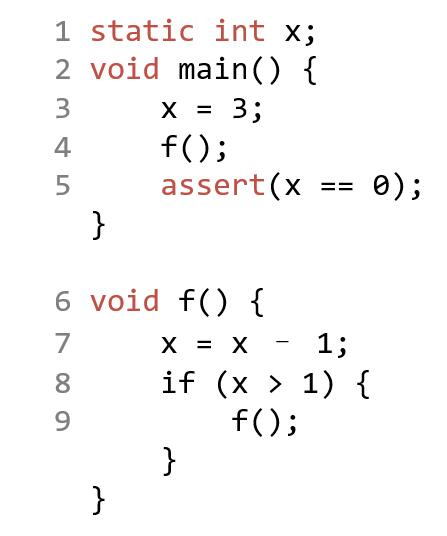
\includegraphics[width=1.7in,height=2in]{Fig3-1.jpg}
\caption{The C program from Figure \ref{fig:BPC}}
\label{fig:FC}
\end{figure}

% 我们将图2-1(a)作为图3-1。在这个错误的C语言程序中,变量x在程序启动时被赋予了初值3,并且程序在完成对函数f的调用后,使用语句assert(x==0)对程序的当前状态进行了断言。
We used Figure \ref{fig:BPC}(a) again, as Figure \ref{fig:FC}. In this faulty $C$ program, variable \lstinline|x| is initialized as \lstinline|3|, and the program uses statement \lstinline|assert(x == 0)| to assert its state after the invocation of function \lstinline|f|.
% 实际上,这两个操作组成了单元测试用例的两个主要元素,即“将程序设置到某个特定的状态”以及“断言程序的最终状态”。
Actually, such operations make up the two basic elements of unit test case, which are "setting the program to a specific initial state" and "asserting the program's final state", or "a known input" and "an expected output" if you prefer.
% 我们给出错误程序的定义:
Here, we give out the basic definition of a faulty program:

\begin{definition}
\label{definition:FaultyProgram}
% 对于布尔程序B,若给定的初始状态使得B在某个assert语句上断言失败,那么我们就说B没能通过由该初始状态和assert语句所断言的最终状态组成的单元测试,即布尔程序B是错误的。
For boolean program $B$, if a given initial state makes $B$ fail to pass some \lstinline|assert| statements, then we say program $B$ doesn't pass the unit test case made up of this initial state and \lstinline|assert| statement,
meaning program $B$ has a fault.
\end{definition}

Also, the definition of a correct program is pretty intuitive:

\begin{definition}
\label{definition:CorrectProgram}
% 正确的程序在运行的过程中总能从初始状态走到程序的正确终止状态且不会经过会使断言失败的错误状态。
A {\it correct} program can always walk from initial state to expected termination state, without passing any wrong state that makes an assertion failed.
\end{definition}

% 在2.1节中,我们将布尔程序的运行图视为了一个有穷自动机。在有穷自动机中,“路径”的概念自然是不陌生的。那么,对于这样的有穷自动机,我们不妨得出其路径的定义如下:
In section \ref{section:SyntaxAndSemanticsOfBooleanProgram}, we describe the control graph of boolean program as a DFA\footnote{Deterministic finite automaton}. No doubt the concept of "path" for DFA should be familiar. In that sense, we define the path of such boolean program DFA as follows:

\begin{definition}
A {\it route} $r$ of boolean program $B$ is an ordered sequence of states $Q_{r}=(q_{r}^{(0)},q_{r}^{(1)},\dots,q_{r}^{(t)})$, in which for any pair of elements $q_{r}^{(i)}$ and $q_{r}^{(i + 1)}$ that makes $i \ge 0$, we have $next(q_{r}^{(i)}) = q_{r}^{(i + 1)}$. In the control graph, a route is represented by a sequence of end-to-end connected edges.
\end{definition}

% 结合定义3.2和定义3.3,我们给出错误路径的定义
With definition \ref{definition:FaultyProgram} and \ref{definition:CorrectProgram}, the definition of bad route can be described as follows:

\begin{definition}
For a route $r$, if there is such state $q_r^{i} = (s,\xi)$ that statement $s$ is an assertion statement and the current evaluation $\xi$ doesn't satisfy this assertion, we say route $r$ is a {\it bad} route.
\end{definition}

\subsubsection{Collecting Bad Routes}
\label{section:CollectingBadRoutes}
% 对于已知的错误语句,我们需要计算出正确的修复语句来进行替换。
For a located faulty statement, we need to produce a correct repairing statement to replace it.
% 我们假设*rep是任意与变量相关的函数,并将*rep作为替换错误语句的表达式,即修复语句。
Assume $*rep*$ is an arbitrary function of all boolean variables, and consider $*rep$ (or the invocation of it) as the repairing statement.
% 替换后,我们便需要去考虑在替换出所延伸出的每种可能路径。
After the replacement, the concrete implementation of $*rep$ is still unknown, hence we need to consider every possible route branches off at this point.

% 假设布尔程序B中只出现了一个*rep。为了计算*rep的恰当实现,我们需要构造该程序的状态转移图。
Assume there is only one $*rep$ in the boolean program $B$. To produce the appropriate implementation of $*rep$, we need to re-construct the state transition graph of this program and every routes branch off at this point
that might lead to wrong termination state.
% 在*rep出现的地方,可以根据它的一个实现从当前状态转移到下一个状态,而它不同的实现则会使当前状态迁移到不同的状态。
When we confronts $*rep$, we can move from one state to another based on one of its possible implementations, and different implementations lead to different states.

% 假设有估值集合,满足:
An implementation of $*rep$ can be considered as a mapping from evaluation to a boolean value (the result of $*rep$). Assume we have a set of evaluations $c \subseteq X$, which satisfies:
\begin{definition}
For any $\xi \in X$, $*rep(\xi) = 1$ if and only if $\xi \in c$. $C = 2^{c}$ is the set of all implementations of $*rep$.
\end{definition}
In other word, $c$ is the set of evaluations which makes $*rep$ return $1$. For each $c$, it would be easy to imagine its corresponding $*rep$ implementation (the mapping).

\begin{figure}
\centering
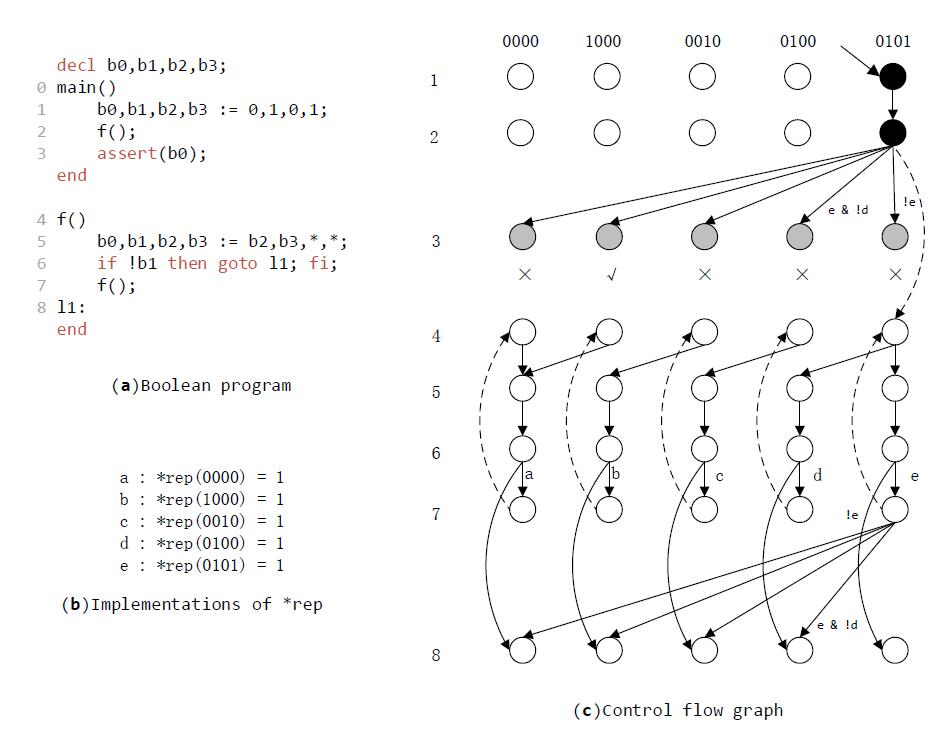
\includegraphics[width=5in,height=3.5in]{Fig3-2.jpg}
\caption{An example of finding all bad routes}
\label{fig:FBR}
\end{figure}

Takes Figure \ref{fig:FBR} as an example, where Figure(a) is basically the same as Figure \ref{fig:BPC}(b).
After replacing the faulty statement with $*rep$, by considering every possible transition corresponding to different $*rep$ implementations,
one can easily draw the control flow graph in \ref{fig:FBR}(c). In this example, we give out predicates $a$, $b$, $c$, $d$ and $e$, representing different elements in evaluation set $c$.
% 以状态(6,00111)为例,程序在此行对*rep函数返回的结果进行判断:若此时函数返回1,即命题e成立,程序进入状态(7,00111)并再次调用函数f;反之,若此时函数返回0,即命题e不成立,程序进入状态(8,00111)并结束函数f。
For example, in state $(6,0101)$, the program will examine the result of function $*rep$: if the function return $1$, meaning predicate $e$ is satisfied, the program will result in state $(7,0101)$ and invoke function \lstinline|f| again; otherwise, if predicate $e$ cannot be satisfied, the program will result it state $(8,0101)$ and return from function \lstinline|f|.
% 假设我们进入了状态(7,00111)并随之来到了状态(6,00110),程序再次对*rep函数返回的结果进行判断:若此时函数返回0,即命题d不成立,程序进入状态(8,00110)并结束函数f。
Assume we enter state $(7,0101)$ and then state $(6,0100)$, the program will examine the result of function $*rep$ again: if the function return $0$, meaning predicate $d$ is unsatisfied, the program will enter state $(8,0100)$ and return from function \lstinline|f|.
% 依此类推,我们就可以计算出main函数从状态(2,00111)分别进入到第三行五个不同状态所需满足的条件。其中,状态(3,10000)、(3,00100)、(3,00110)、(3,00111)均无法通过断言,属于错误状态,其所属的路径便是错误路径。
By repeating this, one can calculate the different requirements for the program to enter the 5 different states in line $3$. Among them, state $(3,0000)$, $(3,0010)$, $(3,0100)$ and $(3,0101)$ cannot pass the assertion, meaning they are wrong termination states, and the routes they belong to are bad routes.

\subsubsection{Producing Repairing Statement}
\label{section:ProducingRepairingStatement}
% 前文的过程可以找到状态转移图中所有连接初始状态和错误终止状态的错误路径。
By constructing all possible routes that lead the program into wrong termination states, we actually find out all wrong implementations of $*rep$.
% 那么不难得出,*rep的正确实现则是这些错误实现所组成的集合的补集。
Then it would be intuitive to know the correct implementation of $*rep$ is the complementary of all these wrong implementations.

\begin{definition}
\label{definition:CorrentREP}
Assume for every implementation $c$ of $*rep$ there is a concrete execution route $r_{c}$, the correct implementation of $*rep$ is $I = C - \{c | \exists q \in r_{c} \wedge q \in bad\}$, where $bad$ is the set of all wrong states.
\end{definition}

% 在上述例子中,我们便收集到了状态(3,10000)、(3,00100)、(3,00110)、(3,00111)所对应的四个错误的*rep实现 ...,即当*rep的实现满足...时,程序将从初始状态进入错误的终止状态。
In the above example, we collect four wrong implementations of $*rep$ corresponding to states $(3,0000)$, $(3,0010)$, $(3,0100)$ and $(3,0101)$: $bcde$, $\cap{c}de$, $\cap{d}e$ and $\cap{e}$,
meaning if the implementation of $*rep$ satisfies $bcde \vee \cap{c}de \vee \cap{d}e \vee \cap{e} = b \vee \cap{c} \vee \cap{d} \vee \cap{e}$, the program will enter wrong state.
% 根据上述定理,我们可以得出正确的*rep实现...,即唯一一条走向正确终止状态(3,01000)的路径。
Based on the above definition, one can safely produce the correct implementation of $*rep$, being $I = \cap{b}cde$, which is also the only route that leads to the correct termination state $(3,1000)$.
% I转换为为此表示并化简后,可得结果...
After representing $I$ with the corresponding predicates and simplifying it based on first-order logic simplification rules, we have $I = \neg b_{0}$.

\subsection{The Satisfiability of the Repairing Statement}
\label{section:TheSatisfiabilityOfTheRepairingStatement}
% 在得出修复公式后,我们还需要考虑该公式是否是可满足的。
After producing the repairing statement, we also need to consider if this statement is satisfiable.

% 布尔程序是对C程序抽象而来,得到布尔程序的修复之后,需要将其重新转换为C语言的修复语句。
Boolean program is abstracted from the original $C$ program. After producing the repairing statement, we also need to convert it back to the corresponding $C$ statement.
% 布尔程序的修复公式,简称布尔修复,是由一系列布尔变量和操作符构成的布尔表达式,其中的布尔变量由C语言程序转换为布尔程序中对原有的变量进行谓词抽象所得,因此布尔修复的每个布尔变量都有着对应的谓词。
The repairing statement for the boolean program, or {\it boolean repair}, is a boolean expression consists of boolean variables and operations, in which all boolean variables are produced by predicate abstraction of the original $C$ program, meaning every boolean variable in the boolean repair has its corresponding predicate.
% 我们应用上一节所述方法得出的布尔修复将会是一个一阶逻辑公式。
The boolean repair produced by the method described in the above section will be a first-order logic expression.
% 由于公式中的每个变量都着其背景理论,公式本身是否可满足是暂不确定的。
As every variable in the expression has its background theory, it is uncertain whether the expression itself is satisfiable.
% 例如图3-2中,谓词p_1的背景理论为x<0,谓词p_2的背景理论为x=0。考虑其背景理论后,实际上公式p_1∧p_2是不可满足的。
For example, in Figure \ref{fig:BPC}, the background theory of predicate $b_{0}$ is $x = 0$, while $b_{2}$ being $x = 1$. Expression $b_{0} \wedge b_{2}$ is clearly unsatisfiable after considering their background theories.
% 由此,我们必须在定义3.6的基础上细化对布尔修复的定义:
In this case, we need to refine the definition of boolean repair based on Definition \ref{definition:CorrentREP}:

\begin{definition}
% 设程序的所有错误路径集合为FP,且...是可满足的,则存在布尔修复使得程序正确,
Assume the set of all bad routes is $FP$, and $\neg (fp_{1} \vee fp_{2} \vee\dots fp_{n}$ is satisfiable, then we say there is a boolean repair that can repair the program.
% 该布尔修复为...,其中bad为程序所有错误状态所组成的集合。
The boolean repair is $I = C - \{c | \exists q \in r_{c} \wedge q \in bad\}$, where $bad$ is the set of all wrong states.
\end{definition}

% 由此,在布尔程序中找到修复公式并不代表能为原本的C语言程序找到修复表达式。
Therefore, existence of a repairing statement for boolean program does not necessarily mean the existence of a corresponding repairing statement for $C$ program.
% 而判断一阶逻辑公式在给定背景理论的情况下是否可满足的问题可以规约到可满足性模理论问题(SMT)
We need to determine if the boolean repair, being a first-order logic expression, is satisfiable after considering the background theories. Such problem can be reduced to the problem of SMT\footnote{Satisfiability modulo theories}\cite{SMT}.

% 我们不妨以析取范式来表示通过本文方法得出的布尔修复,即对于布尔修复φ_rep,有:
As the boolean repair is a first-order logic expression, it would be convenient to first convert it into disjunctive normal form, meaning if we have a boolean repair $\varphi _{rep}$, we have:
\begin{equation}
\varphi _{rep} = \varphi _{1} \vee \varphi _{2} \vee \dots \vee \varphi _{n}
\end{equation}
Every $\varphi _{i}$ is made up of predicate variables and has the following form:
\begin{equation}
\varphi _{i} := p(\tau _{i},\dots,\tau _{n}) | \varphi _{a} \wedge \varphi _{b}
\end{equation}
in which each term $\tau _{i}$ is a $\Sigma$-term (see Equation \ref{eq:SigmaTerm}), representing predicate abstracted from the original $C$ program.
In that sense, one can easily notice that the formula of $\varphi _{rep}$ satisfies the general form of $\Sigma$-formula (see Equation \ref{eq:SigmaFormula}).

% 此外,给定修复公式φ_rep有背景理论T_rep。
Additionally, we assume the background theories of $\varphi _{rep}$ is $T_{rep}$.
% 布尔程序的背景理论均由原C语言程序变量进行谓词抽象得出,因此背景理论T_rep对应修复φ_rep中的谓词变元p(τ_1,τ_2),背景理论的赋值模型与谓词变元的赋值模型一致。
The background theories of boolean program is abstracted from the original $C$ program, hence $T_{rep}$ corresponds to the predicate variable $p(\tau _{1}, \tau _{2})$ in $\varphi _{rep}$, having the same assignment model as predicate variable does.

% 综上,根据先前提到的对可满足性模理论问题的定义,可以证明修复公式φ_rep的可满足性问题都可以规约到可满足性模理论问题。
Above all, based on the definition of SMT shown in former section, one can prove the satisfiability problem of boolean repair $\varphi _{rep}$ can be reduced to SMT.
% 为布尔程序找到的修复公式一定是布尔程序的正确修复,而转换后的φ_rep是否能使C语言程序正确则仍需要进行可满足性判断。
The boolean repair produced by the method describe in the former section is actually the correct repairing statement for the boolean program, but the $\varphi _{rep}$ also has to be satisfiable after conversion.
For now, we know the satisfiability problem of boolean repair $\varphi _{rep}$ can be reduced to SMT, hence we can use the algorithm for SMT to solve the satisfiability program of $\varphi _{rep}$

\subsection{Boolean Repair Simplification}
\label{section:BooleanRepairSimplification}
% 给定析取范式φ,假设存在模型M使得...,即公式φ是可满足的。
For a given DNF\footnote{Disjunctive normal form} expression $\varphi$, assume there is such model $M$ that $M \models \varphi$, meaning expression $\varphi$ is satisfiable.
% 实际上,由于φ是一个析取范式,它的可满足性只能推出它包含可满足的合取子句,但并不能说明它的所有合取子句都是可满足的。
Actually, as $\varphi$ is a DNF expression, all can be inferred from its satisfiability is that it contains satisfiable conjunctive clause, it doesn't mean every clause of it is satisfiable.

% 形式化地说,对于给定的修复公式...,它的可满足并不代表每个φ_i都是可满足的。
Formally speaking, for a repairing statement $\varphi _{rep} := \varphi _{1} \vee \varphi _{2} \vee \dots \varphi _{n}$, it's satisfiability is not sufficient for the satisfiability of every $\varphi _{i}$.
% 例如,对于修复公式...。公式本身是可满足的,因为子句p_3可满足,但子句p_1∧p_2是不可满足的。
For example, consider an repairing statement $\varphi _{rep} := (p_{1} \wedge p_{2}) \vee p_{3}$, where $p_{1} : x > 2, p_{2} : x < 1, p_{3} : x = 0$. The expression is satisfiable as clause $p_{3}$ is satisfiable,
but clause $p_{1} \wedge p_{2}$ is unsatisfiable.

% 若将上例给出的修复公式转换为C语言表达式,我们可以得到C语言修复表达式x>2 && x<1 || x !=0,其中x>2 && x<1部分是没有意义的,该表达式可直接化简为x !=0。
If we convert the expression given in the example to $C$ statement, we have \lstinline{x > 2 && x < 1 || x != 0}, where \lstinline|x > 2 && x < 1| is meaningless, the statement can be simplified to \lstinline|x != 0|.
% 由此可见,我们在将布尔修复转换为C语言表达式前,还需要通过验证其各子句的可满足性来对其进行化简。
Hence, before we convert the boolean repair to $C$ statement, there will be ways to simplify the statement, removing unsatisfiable clauses is one of them.

% 接下来我们将通过三种不同的方式对公式进行化简。
In the following sections, we will use three different ways to simplify the repairing statement.

\subsubsection{Removing Unsatisfiable Clauses}
% 给定可满足的修复公式...,公式子句外的化简是通过判断公式中每个修复子句...的可满足性进行的。
For a given satisfiable repairing statement $\varphi _{rep} := \varphi _{1} \vee \varphi _{2} \vee \dots \vee \varphi _{n}$, one can proceed outer-clause expression simplification by examining the satisfiability of each clause $\varphi _{i}$.
% 如果修复子句φ_i是可满足的,则保留该修复子句;否则,则将其从修复公式φ_rep中移除。
If the clause is satisfiable, the clause should be preserved; otherwise, it can be removed from $\varphi _{rep}$.
% 由3.2节可知,判断子句的可满足性同样可以规约到可满足性模理论问题。
Based on section \ref{section:TheSatisfiabilityOfTheRepairingStatement}, the satisfiability problem of clause $\varphi _{i}$ can also be reduced to SMT.

% 我们将移除不满足修复子句后产生的新的修复公式称为φ_rep^'。
Assume the new repairing statement produced by removing all unsatisfiable clauses are $\varphi _{rep}'$.
% 可以证明,通过子句外化简得到的φ_rep^'和原修复公式φ_rep是等价的,即...。
One can prove $\varphi _{rep}'$ is equivalent to $\varphi _{rep}$, meaning $\varphi _{rep}' \Longleftrightarrow \varphi _{rep}$.

\begin{proof}
% 假设φ_rep^'由φ_rep移除不满足子句φ_i得出,即...
Assume $\varphi _{rep}'$ is produced by removing unsatisfiable clause $\varphi _{i}$ from $\varphi _{rep}$, meaning
\begin{equation}
\label{eq:1}
\varphi _{rep} = \varphi _{rep}' \vee \varphi _{i}
\end{equation}
It should be intuitive that
\begin{equation}
\varphi _{rep}' \Longrightarrow \varphi _{rep}' \vee \varphi _{i}
\end{equation}
Thus,
\begin{equation}
\varphi _{rep}' \Longrightarrow \varphi _{rep}
\end{equation}
We know clause $\varphi _{i}$ is unsatisfiable, meaning $\varphi _{i}$ is always $false$ and $\neg \varphi _{i}$ is always $true$. In this sense, we have
\begin{equation}
\neg \varphi _{i} \wedge (\varphi _{rep}' \vee \varphi _{i}) \Longrightarrow \varphi _{rep}'
\end{equation}
Based on equation (\ref{eq:1}), we have
\begin{equation}
\label{eq:2}
\neg \varphi _{i} \vee \varphi _{rep} \Longrightarrow \varphi _{rep}'
\end{equation}
Given the fact of $\neg \varphi _{i}$ always being $true$, we have
\begin{equation}
\neg \varphi _{i} \wedge \varphi _{rep} = \varphi _{rep}
\end{equation}
Combined with equation (\ref{eq:2}), we have
\begin{equation}
\varphi _{rep} \Longrightarrow \varphi _{rep}'
\end{equation}
\end{proof}

\subsubsection{DNF Simplification}
In this section, we will elucidate how one can proceed inter-clause simplification based on the characteristics of DNF\footnote{Disjunctive normal form}.
A DNF expression can be considered as a tree of clauses, while in the field of computer algorithm, tree-like structure is simplified mostly by rule-based methods.
Several general and effective simplification rules will be listed and proved below accordingly.

\begin{theorem}
For a given satisfiable expression $\varphi = p \vee (q \wedge r)$, if $p \vee r$ or $p \vee q$ always being $true$, $\varphi$ can be simplified to be $p \vee q$ or $p \vee r$ respectively.
\end{theorem}
One can prove this theorem easily based on the distribution law of first-order logic.

\begin{theorem}
For a given satisfiable expression $\varphi = (\varphi _{1} \wedge q) \vee (\varphi _{2} \wedge \neg q) \vee \varphi _{other}$, if every predicate in $\varphi _{1}$ is also contained in $\varphi _{2}$,
$\varphi$ can be simplified to be $\varphi = (\varphi _{1} \wedge q) \vee \varphi _{2} \vee \varphi _{other}$.
\end{theorem}
\begin{proof}
Each clause $\varphi _{i}$ is actually made up of conjunction of predicates. As every predicate in $\varphi _{1}$ is contained in $\varphi _{2}$, we have $\varphi _{2} = \varphi _{1} \wedge \varphi _{3}$,
where $\varphi _{3}$ consists all predicates that are in $\varphi _{2}$ but not in $\varphi _{1}$. Then we have
\begin{equation}
(\varphi _{1} \wedge q) \vee (\varphi _{2} \wedge \neg q) = (\varphi _{1} \wedge q) \vee (\varphi _{1} \wedge \varphi _{3} \wedge \neg q)
\end{equation}
It can be further transformed into the following by using distribution law:
\begin{equation}
(\varphi _{1} \wedge q) \vee (\varphi _{1} \wedge \varphi _{3} \wedge \neg q) = ((\varphi _{1} \wedge q) \vee (\varphi _{1} \wedge \varphi _{3})) \wedge ((\varphi _{1} \wedge q) \vee \neg q)
\end{equation}
in which the $(\varphi _{1} \wedge q) \vee \neg q$ part on the right hand side can be simplified by further use of distribution law:
\begin{equation}
(\varphi _{1} \wedge q) \vee \neg q = (\varphi _{1} \vee q) \wedge (q \vee \neg q) = \varphi _{1} \wedge \neg q
\end{equation}
Therefore,
\begin{equation}
\begin{tabular}{rcl}
$(\varphi _{1} \wedge q) \vee (\varphi _{1} \wedge \varphi _{3} \wedge \neg q)$&$=$&$((\varphi _{1} \wedge q) \vee (\varphi _{1} \wedge \varphi _{3})) \wedge (\varphi _{1} \vee \neg q)$ \\
                                                                               &$=$&$((\varphi _{1} \wedge q) \wedge (\varphi _{1} \vee \neg q)) \vee ((\varphi _{1} \wedge \varphi _{3}) \wedge (\varphi _{1} \vee \neg q))$ \\
\end{tabular}
\end{equation}
in which the $(\varphi _{1} \wedge q) \wedge (\varphi _{1} \vee \neg q)$ part on the right hand side can be simplified by using association law:
\begin{equation}
(\varphi _{1} \wedge \varphi _{3}) \wedge (\varphi _{1} \vee \neg q) = \varphi _{1} \wedge \varphi _{3} = \varphi _{2}
\end{equation}
Hence,
\begin{equation}
\begin{tabular}{rcl}
$(\varphi _{1} \wedge q) \vee (\varphi _{1} \wedge \varphi _{3} \wedge \neg q)$&$=$&$(\varphi _{1} \wedge q) \vee \varphi _{2}$ \\
$(\varphi _{1} \wedge q) \vee (\varphi _{2} \wedge \neg q)$&$=$& \\
\end{tabular}
\end{equation}
By such mean, we proved the theorem after adding $\varphi _{other}$ on both sides:
\begin{equation}
(\varphi _{1} \wedge q) \vee (\varphi _{2} \wedge \neg q) \vee \varphi _{other} = (\varphi _{1} \wedge q) \vee \varphi _{2} \vee \varphi _{other}
\end{equation}
\end{proof}

The simplification rules listed above are just two examples.
No doubt, adding more rules can enhance the accuracy of this algorithm,
but judging from experimental results, these two rules are already effective enough for most cases.

\subsubsection{Simplification based on Background Theories}
Let's start this section with a simple example: assume we have a simplified repairing expression $\varphi _{rep} = p _{1} \vee p _{2}$ after applying the methods described in former sections,
where $p _{1}$ is \lstinline|x < 2| and $p _{2}$ is \lstinline|x < 3|. The corresponding $C$ statement of $\varphi _{rep}$ would be \lstinline{x < 2 || x < 3}, which can still be simplified to be \lstinline|x < 3|.
In this sense, simplification based on background theories, or inner-clause simplification, is necessary to produce a simplified and intuitive $C$ statement.

\begin{theorem}
\label{theorem:1}
For a given simplified repairing expression $\varphi _{rep} = p \wedge q \wedge \varphi$ and the corresponding background theory $T$, if there is a binary predicate $r = p \wedge q$ in $T$,
repairing expression $\varphi _{rep}$ can be simplified to be $\varphi _{rep} = r \wedge \varphi$.
\end{theorem}
\begin{theorem}
\label{theorem:2}
For a given simplified repairing expression $\varphi _{rep} = p \vee q \vee \varphi$ and the corresponding background theory $T$, if there is a binary predicate $r = p \vee q$ in $T$,
repairing expression $\varphi _{rep}$ can be simplified to be $\varphi _{rep} = r \vee \varphi$.
\end{theorem}

Theorem \ref{theorem:1} and \ref{theorem:2} is related to the background theory $T$, where the predicate $r$ from $T$ may be new from $p$ and $q$ or one of them.
As the repairing expression will always be in DNF, these two simplification rules are actually sufficient.

\subsection{Summary}
In this section, we illustrated the basic work flow of $C$ program automatic repair. In section \ref{section:BooleanProgramRepair}, we introduced the basic concept of producing boolean repair by collecting bad routes for converted boolean program,
while section \ref{section:TheSatisfiabilityOfTheRepairingStatement} focuses on reducing the satisfiability problem of the boolean repair to SMT. We demonstrated some basic rules of simplifying the boolean repair in section \ref{section:BooleanRepairSimplification}, and by such way we eventually produce an effective and intuitive $C$ repairing statement for the original $C$ program.
